% 1977 年内蒙古卷理科第 2(1) 题：梯形对角线与平行截线
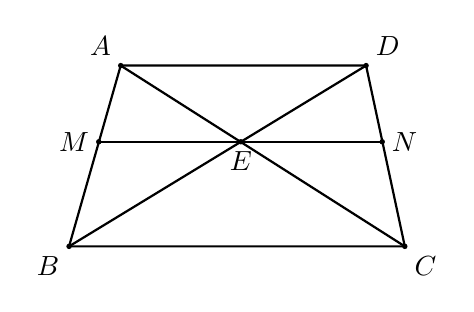
\begin{tikzpicture}[scale=0.82]
  \coordinate (A) at (0.8,2.8);
  \coordinate (D) at (4.6,2.8);
  \coordinate (B) at (0,0);
  \coordinate (C) at (5.2,0);
  \coordinate (E) at (2.66,1.62);
  \coordinate (M) at (0.46,1.62);
  \coordinate (N) at (4.85,1.62);
  \draw[thick] (A)--(D)--(C)--(B)--cycle;
  \draw[thick] (A)--(C);
  \draw[thick] (B)--(D);
  \draw[thick] (M)--(N);
  \fill (A) circle (1.2pt) node[above left] {$A$};
  \fill (D) circle (1.2pt) node[above right] {$D$};
  \fill (B) circle (1.2pt) node[below left] {$B$};
  \fill (C) circle (1.2pt) node[below right] {$C$};
  \fill (E) circle (1.2pt) node[below] {$E$};
  \fill (M) circle (1.2pt) node[left] {$M$};
  \fill (N) circle (1.2pt) node[right] {$N$};
\end{tikzpicture}
